\documentclass{standalone}
\usepackage{tikz}
%\usetikzlibrary{...}
\begin{document}
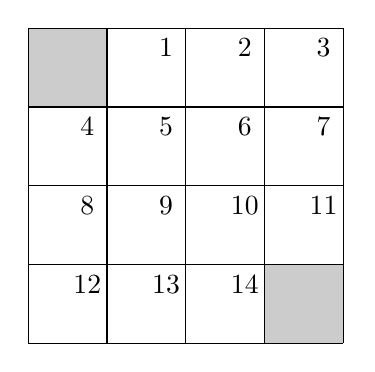
\begin{tikzpicture}
  \begin{scope}[local bounding box=L]
 \fill[black!20] (0,3) rectangle ++ (1,1); 
 \fill[black!20] (3,0) rectangle ++ (1,1); 
 \draw (0,0) grid (4,4); 

 \node at (1.75,+3.75) {1};
 \node at (2.75,+3.75) {2};
 \node at (3.75,+3.75) {3};
 
 \node at (0.75,+2.75) {4};
 \node at (1.75,+2.75) {5};
 \node at (2.75,+2.75) {6};
 \node at (3.75,+2.75) {7};
 
 \node at (0.75,+1.75) {8};
 \node at (1.75,+1.75) {9};
 \node at (2.75,+1.75) {10};
 \node at (3.75,+1.75) {11};
 
 \node at (0.75,+0.75) {12};
 \node at (1.75,+0.75) {13};
 \node at (2.75,+0.75) {14};

\end{scope} 
\end{tikzpicture}
\end{document}
